% -*- mode: LaTex; outline-regexp: "\\\\section\\|\\\\subsection";fill-column: 80; -*-
\documentclass[12pt]{article}
\usepackage[longnamesfirst]{natbib}
\usepackage[usenames]{color}
\usepackage{graphicx}  % Macintosh pdf files for figures
\usepackage{bbm}       % one symbol
\usepackage{amssymb}   % Real number symbol {\Bbb R}
\input{../../standard}

% --- margins
\usepackage{../../sty/simplemargins}
\setleftmargin{1in}   % 1 inch is NSF legal minimum
\setrightmargin{1in}  % 1 inch is NSF legal minimum
\settopmargin{1in}    % 1 inch is NSF legal minimum
\setbottommargin{1in} % 1 inch is NSF legal minimum

% --- Paragraph split, indents
\setlength{\parskip}{0.00in}
\setlength{\parindent}{0in}

% --- Line spacing
\renewcommand{\baselinestretch}{1.3}

% --- Margins
\setlength{\topmargin}{-0.5in}
\setlength{\oddsidemargin}{-0.1in}
\setlength{\textheight}{9.0in}
\setlength{\textwidth}{6.5in}

% --- page numbers
\pagestyle{empty}  % so no page numbers

% --- Hypthenation
\sloppy  % fewer hyphenated
\hyphenation{stan-dard}
\hyphenation{among}

% --- Customized commands, abbreviations
\newcommand{\TIT}{{\it  {\tiny Risk of sequential tests (\today)}}}

\newcommand{\test}{\mbox{$\hat\mu(\al(\cdot),w_0,\omega)$}}
\newcommand{\uTest}{\mbox{$\hat\mu(\al_u(\cdot),w_0,\omega)$}}
\newcommand{\gTest}[1]{\mbox{$\hat\mu(\al_g(\cdot,{#1}),w_0,\omega)$}}

% --- Header
\pagestyle{myheadings}
\markright{\TIT}

% --- Title

\title{ Risk of Sequential Testing with Alpha Investing }
\author{
        Dean P. Foster and Robert A. Stine
        \thanks{Research supported by NSF grant DMS-1106743 }  \\
        Department of Statistics            \\
        The Wharton School of the University of Pennsylvania \\
        Philadelphia, PA 19104-6340                          \\
        www-stat.wharton.upenn.edu/$\sim$stine 
}

\date{\today}


%%%%%%%%%%%%%%%%%%%%%%%%%%%%%%%%%%%%%%%%%%%%%%%%%%%%%%%%%%%%%%%%%%%%%%%%%%%

\begin{document}
\maketitle 
%------------------------------------------------------------------------

\abstract{ 

 Streaming feature selection evaluates potential explanatory variables
 sequentially rather than all at once.  This approach provides adaptive control
 of the scope of a search for predictive features and makes it possible to
 consider large collections of features.  It also produces novel challenges for
 variable selection.  Methods such as alpha investing can be used to control the
 rate of false discoveries, but little is known about the risk of the resulting
 estimator.  We provide a computational framework that determines the
 nonasymptotic minimax risk of a sequential estimator relative to an
 alternative.  The alternative can be data driven or supported by an oracle.
  Our findings demonstrate that in all but very sparse models, estimators
 allowed to have larger rates of false discoveries produce smaller risk.

}

%------------------------------------------------------------------------
\vspace{0.05in}

\noindent
{\it Key Phrases: Bellman equations, dynamic programming, streaming feature
 selection, testimator, variable selection}

\clearpage


% ----------------------------------------------------------------------
\section{ Introduction }
% ----------------------------------------------------------------------

This paper shows one of the powerful advantages of using a streaming
feature selection approach.  If we consider figure 1 (where figure 1
is one of the convex set) we can see how two estimators compare based
on their risk performance.  Such graphs are common (cite...) but
typically can only be generated for very specific pairs of estimators.
Using a Bellman approach, we can easilly generate such figures for
any pair of streaming feature selection methods.   These are finite
sample figures which are exact in the sense that every point in the
convex set can be achieved by some probabilistic mode

 Streaming feature selection constructs a predictive model by choosing
 explanatory variables from a sequence offered by an exogenous source.  Rather
 than evaluate these variables simultaneously, streaming selection evalutes them
 one-at-a-time.  Greedy searches like stepwise regression consider the full
 batch of, say, $p$ potential explanatory variables together, choosing at the
 first step the predictor $X_{(1)}$ that obtains the best fitting model.  In
 contrast, streaming selection evaluates the offered predictors sequentially as
 $X_1, \, X_2, \ldots$, performing the evalation of $X_j$ in the context of the
 model produced by picking from $X_1, \ldots, X_{j-1}$.  Hence, streaming
 selection does not require the full set of explanatory variables at the start
 of the search and is free to use the results of evaluating initial variables to
 guide the search for those to add subsequently.  For example, if it adds $X_j$
 to the model, the streaming search might then be expand add interactions $X_j
 \, X_k$ to the queue of possible variables to consider.  Streaming selection
 can thus rapidly explore collections of explanatory variables that are larger
 than typically considered with conventional methods; the slowest step in
 forward stepwise regression is the calculation of the $X'X$ matrix.
  \citet{fosterlin10} show examples selecting from up to $p$=100,000 explanatory
 variables.


 Streaming selection poses a challenge, however, for variable selection.
  Although it is advantageous to avoid simultaneously evaluating every
 predictor, the absence of a fixed set of features in streaming selection
 requires a different type of selection criterion from those commonly used.  For
 example, suppose the search begins with a list of $p$ possible features $X_1,
 X_2, \ldots, X_p$.  As mentioned previously, the search could expand to include
 interactions in $X_j$ once $X_j$ joins the model.  If the search is limited to
 second-order interactions (one could allow higher order interactions as well),
 then the maximum number of possible explanatory variables is $m = p(p+1)/2$
 variables.  Since few of these would be considered, it would be very
 conservative to combine $m$ with a criterion such as AIC, BIC, or RIC.
  Similarly, selection using FDR requires the full set of marginal $p$-values.


 Alpha investing \citep{fosterstine08} is a sequential testing procedure
 designed to support streaming feature selection.  Because alpha investing can
 test an infinite sequence of hypotheses, it is well-matched to a search of an
 unbounded collection of features that is too large to manipulate
 simultaneously.  Rather than test multiple hypotheses at once, alpha investing
 tests hypotheses one-at-a-time in a specified order.  Alpha investing begins
 with an initial allowance for Type I error that is called its alpha wealth.
  Each test consumes some of the available alpha wealth, as in the alpha
 spending rules used in clinical trials.  Alpha investing differs from these and
 overcomes the conservatism of alpha spending rules, which include the
 Bonferroni method, by earning a contribution to the alpha wealth available for
 subsequent tests for each rejected null hypothesis.  Thus rejections beget more
 rejections.  Alpha investing further allows one to test an infinite stream of
 hypotheses, accommodate dependent tests, and incorporate domain knowledge.
 

 Though flexible, alpha investing controls the expected number of false
 rejections.  Controlling the false discovery rate with alpha investing guards
 against overfitting in variable selection.  With alpha inveseting, one can
 guarantee that on average not more than, say, 5\% of the rejected hypotheses
 spuriously add a predictor to the model.  When building a predictive model,
 however, controlling the false discovery rate is frequently secondary to
 obtaining a more predictive model.  Control of the false discovery rate does
 not imply that one will find the most predictive model possible.  It only
 guarantees that a high percentage of chosen features are in fact useful.  The
 risk of the implied estimator is more relevant.


 Our analysis considers the cumulative risk of a sequence of testimators implied
 by testing a sequence of null hypotheses.  A testimator is also known as a
 keep-or-kill estimator or a hard thresholding estimator.  The estimator of a
 parameter $\mu$ is zero unless a test of the null hypothesis that claims $\mu =
 0$ is rejected.  The estimation problem we consider is a simplified version of
 the variable selection problem that avoids issues related to the collinearities
 among the explanatory variables.  Rather than observe a sequence of slope
 estimates, we assume that the observed data are a finite sequence of $p$ random
 variables $Y_j \sim N(\mu_j,1)$.

 Mention: stochastic dynamic programming, no discounting because of the finite
horizon, 

 \ras{ Revise roadmap paragraph }
 The following section describes the use of alpha-investing for setting the
 levels $\al_j$ of the tests that determine the testimator $\hat\mu$.  Section 3
 describes the computations that solve a set of Bellman equations.  Our
 methodology bounds the risk of any sequential testimator.  In the spirit of
 risk inflation and oracle bounds, we compute the convex set of attainable
 risks:
 \begin{equation}
   \CC(\hat\gamma) 
      = \{(x,y): \exists \mu \mbox{ for which }
                 x=R(\tilde\mu,\mu), \, y = R(\hat\mu_{\hat\gamma},\mu)\} \;,
 \label{eq:C}
 \end{equation}
 where $\tilde\mu$ identifies an oracle estimator of $\mu$ that is defined in
 Section 3.  The boundary of $\CC$ produces exact results that are comparable to
 those obtained in asymptotic multivariate setting.  Section 4 displays the risk
 of these procedures, and we conclude with a summary and discussion of open
 issues in Section 5.


% ---------------------------------------------------------------------------
\section{ Alpha-investing }
% ---------------------------------------------------------------------------

 An alpha-investing rule \citep{fosterstine08} determines the level for testing
 $H_j$ based on its alpha wealth, a limit on the maximum level that depends on
 the results of prior tests.  The procedure is most easily described by
 explaining the first few steps.  The process begins with an initial allocation
 $w_0$ \marginpar{$w_0$} of alpha wealth.  The choice of this initial alpha
 wealth is an important aspect of our analysis of the risk of $\hat\mu$.  An
 alpha-investing rule can test $H_1$ at any level up to the total available
 alpha wealth, $0 \le \alpha_1 \le w_0$.  The level $\al_1$ is `invested' and
 cannot be used for subsequent tests.  We say that $\al_1$ is invested rather
 than spent because of the way in which the outcome of the test of $H_1$
 influences the subsequent wealth.  Let $p_1$ denote the p-value of the test of
 $H_1$.  If $p_1 \le \alpha_1$, the test rejects $H_1$.  In this case, the
 alpha-investing rule earns a contribution $\omega > 0$ \marginpar{$\omega$} to
 its alpha wealth; otherwise, the alpha wealth available to test $H_1$ falls to
 $W_1 = w_0 - \alpha_1$.  In general, the alpha wealth available for the test of
 $H_{j+1}$ is given by the stochastic process \marginpar{$W_j$}
 \begin{equation}
    W_j = W_{j-1} - \alpha_j + \omega \, I_{\{p_j < \al_j\}}, \; j = 1,\,2,\ldots,
 \label{eq:Wj}
 \end{equation}
 with the initial condition $W_0 \equiv w_0$.  Alpha investing thus resembles
 alpha spending used in clinical trials, with the key distinction that rejecting
 a hypothesis earns an additional allocation $\omega$ of alpha-wealth for
 subsequent testing.  \ras{reference to QPD and enhanced alpha investing}


 Because rejecting a null hypothesis makes it easier to reject other null
 hypotheses, it is important that alpha investing controls the rate of false
 rejections.  To this end, \citet{fosterstine08} show that alpha investing
 controls a sequential version of mFDR.  Let $D(j)$ count the number of
 hypothesis rejected in the first $j$ tests, and let $V(j) \le D(j)$ denote the
 number of {\em false} rejections through the first $j$ tests.  The sequential mFDR is
 \begin{equation}
    \mbox{mFDR}_\eta(j) = \frac{\ev V(j)}{\eta + \ev R(j)} \;, \eta > 0.
 \label{eq:mFDR}
 \end{equation}
 The similar false discovery rate is essentiallyt the expected value of the
 ratio rather than the ratio of expected values.  The constant $\eta$ in the
 denominator of mFDR avoids dividing by zero under the complete null hypothesis
 in which all $\mu_j = 0$.  If $w_0 \le \omega$, then alpha-investing rules
 control $\mbox{mFDR}_\eta(p) \le \omega$, and this result implies weak control
 of the family wide error rate.  Furthermore, the index $j$ in \eqn{eq:mFDR} is
 allowed to be an arbitrary stopping time, such as the occurrence of the $k$th
 rejection.

 
 Alpha-investing rules are quite general.  The underlying theory requires only
 that the level of the test of $H_j$ is bounded by the available wealth
 $W_{j-1}$ and that the test indeed have level $\al_j$, conditional on the
 outcomes of prior tests.  Otherwise, an alpha-investing rule is allowed to use
 the pattern of prior rejections as captured by the sequence of wealths.  We can
 capture this dependence by thinking of the investing rule ${\cal A}$ as a
 function of the sequence of prior wealths $W_0^j = \{W_0, W_1, \ldots, W_j\}$.
  A rule is then a map from the sequence of wealths to a number on the interval
 0 to the current wealth:
 \begin{equation}
    {\cal A}: W_0^j \mapsto [0, \min(W_j,1)]    
 \label{eq:A}
 \end{equation}
 For example, the rule $\cal A$ can set the wealth of the next test higher or
 lower depending upon how long since the last rejection or the number of
 rejections to this point.  Though alpha investing allows this complete
 generality, we focus our attention on a simpler class of investing rules with a
 path independent, Markovian structure.  The amount invested by these rules
 depends only on the current wealth rather than the full path, ${\cal A}(w_0^j)
 = \al(W_j)$.  The only requirement is that $0 \le \al(w) \le w$; a rule cannot
 invest more wealth than the amount possessed.  It does seem natural, however,
 for $\al(w)$ to be monotone increasing in $w$.


 The simplest representatives of this class of alpha investing rules are
 geometric rules.  These invest a fixed percentage of the available wealth on
 each test:
 \begin{equation}
    \al_g(w, \psi) = \psi \, w, \quad  0 < \psi < 1.
 \label{eq:Ageo}
 \end{equation}
 Though independent of the rejection path, geometric rules invest more heavily
 following a rejection.  Since the alpha wealth increases after a rejection, a
 geometric rule $\al_g$ invests more following a rejection and then gradually --
 depending on $\psi$ -- reduces the level of subsequent tests.


 The following investing rule varies the invested share.  Rather than investing
 a fixed share of the available wealth, it invests a progressively smaller share
 of the available wealth as the wealth drops.  The rule is defined by
 \begin{equation}
   \al_u(w) = w - \frac{\log 2}{\log(1+2^{1/w})} \;.   
 \label{eq:Auniv}
 \end{equation}
 Because this investing rule is related to the universal prior for integers
 defined by \citet{rissanen83}, we call this a universal investing rule and
 identify it by a subscript $u$.  (See the following remark.)  For very large
 wealth, $\al_u(w)$ approaches $w$ (the limit of the second term in
 \eqn{eq:Auniv} is $w-1$ as $w \rightarrow \infty$), and $\al_u(w)
 \rightarrow 0$ as $w \rightarrow 0$.

 
 Figure \ref{fig:rules} contrasts the investments produced by the universal and
 several alpha investing rules on a log-log scale.  The initial wealth for all
 rules is set to $w_0 = 1$.  With this scaling, the amounts invested by the
 universal rule falls off approximately linearly.  The amounts invested by the
 universal rule are initially larger than those of any of these geometric rules.
  With $w_0=1$, the universal rule invests about $0.369$, $0.131$, $0.0693$,
 $0.0438$, and $0.0306$ in the first five tests before its spending gradually
 slows. After this initial period, each geometric rule has a range of tests over
 which the geometric rule provides a larger alpha level for testing $H_j$ than
 the universal rule.  Ultimately, however, each geometric rule invests smaller
 amounts than the geometric rule as the testing continues.  For example, the
 geometric rule that invests 1\% of its current wealth at each test
 ($\psi=0.01$) invests more than the universal rule when testing $H_{11}$
 through $H_{581}$. \ras{ Say more here about why this 'blending' of the
 geometric rates is a good thing; too bad we don't have that 'habitation' idea
 worked out where the universal finds a steady rate appropriate for the rate of
 false nulls. }


 \begin{figure}
 \caption{ \label{fig:rules} \sl Investments for the universal and several
 geometric alpha investing rules if no intervening test rejects. }

 \centerline{
 \vspace{0.1in}
 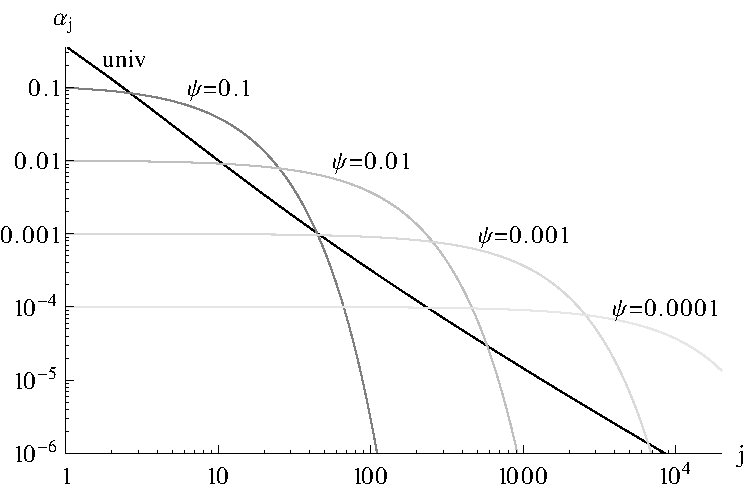
\includegraphics[width=3.5in]{figures/rules} }
 \vspace{0.2in}
 \end{figure}


 \remark{ We obtained the universal rule by the following construction
 that links a spending rule to a probabilty distribution that allocates the
 current wealth over subsequent tests.  }

We illustrate the construction for the geometric rule.  If the initial wealth
 is $w_0$, then the alpha wealth invested in the $j$th test (assuming no
 intervening test rejects) is
 \begin{equation}
    \al_j = w_0\; \psi \; (1-\psi)^{j-1} \;, \quad j = 1, 2, \ldots\;.   
 \label{eq:alj1}
 \end{equation}
  Rather than define the investing rule using a discrete distribution on
 $j=1,\,2,\ldots$ as in \eqn{eq:alj1}, use the continuous density
 \begin{equation}
   A_g(x,\psi) = c_g \; \psi\,(1-\psi)^{x-1}, \quad 1 \le x\;,
 \label{eq:alg}
 \end{equation}
 where the normalizing constant $c_g = -\log (1-\psi)/\psi$.  Notice that the
 wealth invested in the $j$th test \eqn{eq:alj1} matches the integral of
 $A_g(x)$ from $x=j$ to $x=j+1$,
 \begin{equation}
    \al_j = w_0 \int_j^{j+1} A_g(x,\psi) dx = w_0 \, \psi\; (1-\psi)^{j-1} \;.
 \label{eq:alj2}
 \end{equation}
 To move away from this discrete indexing, note that the following tail integral
 shows the amount of wealth that remains,
 \begin{equation}
    W_g(x) = w_0 \int_x^\infty A_g(t,\psi) dt = w_0 (1-\psi)^{x-1}\;.
 \label{eq:Wg}
 \end{equation}
 For integers $j$, $W_g(j)$ is the wealth remaining after $j$ tests that fail to
 reject.  By inverting this tail integral, we obtain an investing rule that
 requires only the available wealth,
 \begin{equation}
   \al_g(w,\psi) = A_g(W_g^{-1}(w),\psi) = \psi\,w \;,
 \label{eq:Ag}
 \end{equation}
 as in \eqn{eq:Ageo}.  This construction uses the inverse of the tail wealth to
 determine a `test index' $W_g^{-1}(w)$ that corresponds to the current input
 wealth $w$.  The universal rule $\al_u(w)$ follows from the same
 contruction, with the density
 \begin{displaymath}
    A_u(x) = \frac{\log 2}{(x+1) (\log(x+1))^2} \;, \quad 1 < x,
 \end{displaymath}
 used in place of $A_g$.

 \remark{ To avoid adding notation, we overload the symbol $\al$.  By
 itself, we use $\al$ to represent the generic level of a test.  When given an
 integer subscript, $\al_j$ is the level of the $j$th test in sequence of tests,
 as in \eqn{eq:alj1}.  Finally, when denoting a function, $\al(w)$ is the level
 invested in a test by a procedure that has available wealth $w$, as in
 \eqn{eq:Ageo} or \eqn{eq:Auniv}.  Throughout these uses, the symbol $\alpha$
 consistently gives the level of a test; only the context of the test changes.}


%--------------------------------------------------------------------------
\section{ Risk Analysis}
%--------------------------------------------------------------------------

 We start by considering the risk of testimators in the case of a single test or
 multiple simultaneous tests.  This foundation allows us to introduce the
 approach that we take when studying the risk produced by alpha investing
 procedures in the sequential context.


 We first consider the squared error risk of testimators for a single parameter.
  Let $Y \sim N(0,1)$.  The scalar testimator defined by the two-sided test of
 $H_0: \mu=0$ at level $\al$ is
 \begin{equation}
   \hat\mu_\al(Y) = \left\{
     \begin{array}{cc}
        Y & \mbox{ if } z_\al^2 \le Y^2, \cr
        0 & \mbox{ otherwise, }
      \end{array} \right.
 \label{eq:muHat}
 \end{equation}
 where $z_\al$ denotes the positive, two-sided critical value
 \begin{equation}
   z_\al = \Phi^{-1}(1-\al/2) \;.
 \label{eq:zAlpha}
 \end{equation}
 The risk of $\hat\mu_\al$ is
 \begin{eqnarray}
   R(\hat\mu_\al(Y), \mu) 
     &=& \ev(\hat\mu_\al(Y) - \mu)^2  \cr
     &=& \mu^2 \pr(Y^2 \le z_\al^2) 
         + \int_{y^2>z_\al^2} (y-\mu)^2 \phi(y) dy \cr
     &=& B_\al(\mu) + V_\al(\mu)
 \label{eq:risk_mu_al}
 \end{eqnarray}
 The first summand $B_\al(\mu)$ is the squared bias that arises if the test of
 $H_0: \mu=0$ does not reject when $\mu \ne 0$; the second summand is the
 variance of the estimator.  Figure \ref{fig:risk}(a) shows a graph of the risk
 of testimators with $\al=0.05$ and $\al = 0.20$.  The maximum risk that occurs
 near $z_\al$ grows as the level $\al$ shrinks.  Figure \ref{fig:risk}(b) shows
 the decomposition of the risk of $\hat\mu_\al$ into $B_\al(\mu)$ and
 $V_\al(\mu)$ for $\al = 0.05$.  Because the variance component $V_\al(\mu)$
 increases smoothly to its maximum 1 for large $|\mu|$, it is the bias that
 produces the noticeable peak that identifies the maximum risk just outside
 $z_\al$.


 \begin{figure}
 \caption{ \label{fig:risk} \sl Risk of testimators. (a) Risk of testimators with
 $\al$ = 0.05, 0.20 versus $\mu$. (b) Squared bias and variance components of the
 risk of $\hat\mu_{0.05}$. } 
 \vspace{0.1in}
\centerline{
 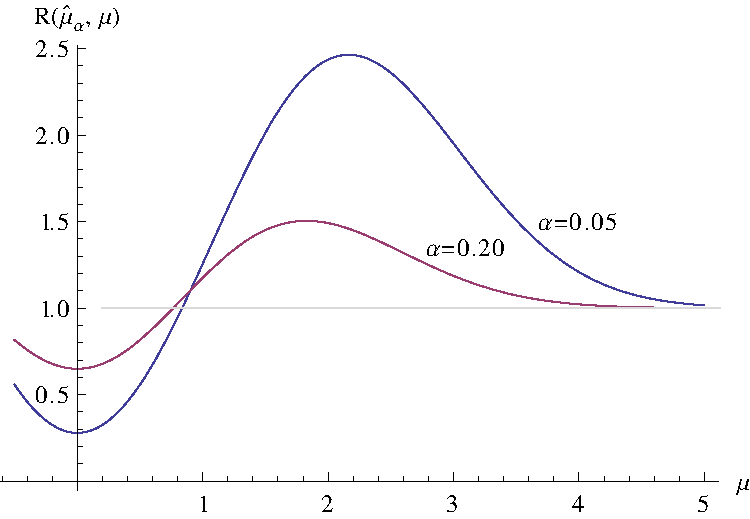
\includegraphics[width=3.0in]{figures/risk_a}
 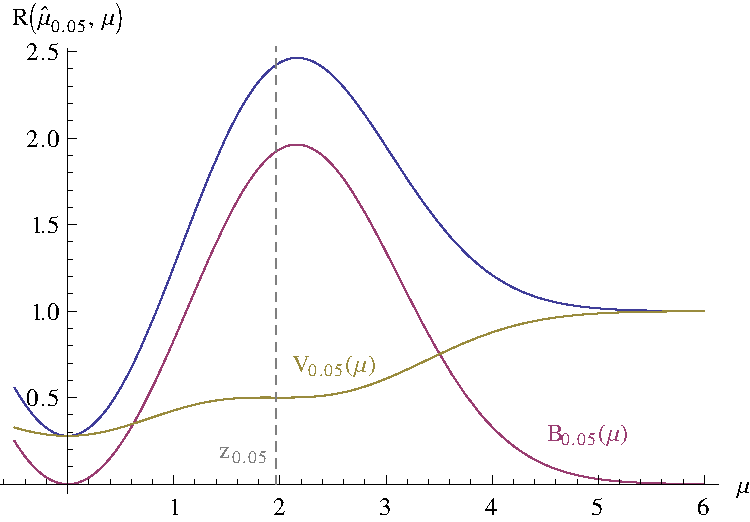
\includegraphics[width=3.0in]{figures/risk_b} }
 \vspace{0.2in}
 \end{figure}
 

 The analysis of the risk of testimators is typically done in the context of
 estimation a vector of $p$ means, $\bmu \equiv \mu_{1:p} =
 (\mu_1,\ldots,\mu_p)'$.  The available data is the vector $\YY \equiv Y_{1:p} =
 (Y_1, \ldots, Y_p)'$ with distribution $\YY \sim N(\bmu,I_p)$.  The estimator
 of $\bmu$ combines testimators at a common level in each coordinate,
 $\hat{\bmu}_\al = (\hat\mu_\al(Y_1), \ldots, \hat\mu_\al(Y_p))'$.  The estimator
 $\hat{\bmu}_\al$ consists of zeros except for those coordinates where $z_\al^2
 \le Y_j^2$.  The risk of $\hat{\bmu}_\al$ is the sum of the risks of the
 coordinate testimators,
 \begin{equation}
    R(\hat{\bmu}_\al, \bmu) 
      = \ev\; \normsq{\hat{\bmu}_\al - \bmu} \;,
 \label{eq:risk}
 \end{equation}
 where $\normsq{x} = x'x$ for vectors $x$.  We note that our notation suppresses
 the dependence of the estimator $\hat{\bmu}_\al(\YY)$ on the data.  The full
 vector $\YY$ is available for setting the level as well.


 Minimax bounds for the risk $R(\hat{\bmu}_\al,\bmu)$ are well-understood.  We briefly
 review the results of \citet{fostergeorge94} who introduced the concept of the
 risk inflation of an estimator. \citep[][obtain similar results.]
  {donohojohnstone94} The risk inflation of $\hat{\bmu}_\al$ is the supremum of
 the ratio of the risk of the testimator $\hat{\bmu}_\al$ at level $\al$ to the
 risk of a testimator that obtains the optimal level from an oracle. 
  Their results imply that the risk inflation of $\hat{\bmu}_\al$ is
 asymptotically $2 \log p$,
 \begin{equation}
    2 \log p - o(\log p) 
    \le
    \sup_\mu  \frac{1 + R(\hat{\bmu}_\al,\bmu)}
                   {1 + \inf_\eta{R(\hat{\bmu}_\eta,\bmu)}}  
    \le 
    2 \log p + 1 \;.
 \label{eq:ri}
 \end{equation}
 Foster and George further show that the testimator $\hat{\bmu}_{1/p}$ --
 essentially the Bonferoni estimator -- obtains the risk inflation threshold.
  The constant 1 added to the risks in the ratio of \eqn{eq:ri} arises in the
 context of regression models in which one always estimates the intercept.  As a
 practical device, its presence in the denominator avoids dividing by zero under
 the complete null model in which $\mu_j = 0$ for all $j$.


 Though suggestive, these results do not reveal the risk of the testimator
 derived from alpha investing.  The key difference lies in the timing of the
 choice of the test levels.  The testimator studied in risk inflation
 $\hat{\bmu}_\al$ uses a fixed level $\al$ for all $p$ coordinates, and all of
 the elements of \YY are used to set this common level.  In sequential testing,
 the $Y_j$ are observed sequentially so that the elements of the estimator form
 a stochastic process, which we collect in a $p$-element vector as
 \begin{equation}
   \hat\mu(\al(\cdot),w_0,\omega) = (\hat\mu_{\al(w_0)}, \hat\mu_{\al(W_1)}, \ldots, 
                       \hat\mu_{\al(W_{p-1})})',
 \label{eq:muHatAlphaInv}
 \end{equation}
 where $\al(\cdot)$ denotes the defining investing rule, $w_0$ is the initial
 alpha wealth, and $\omega$ is the payout earned when rejecting a hypothesis.
  The wealth random variables $W_j$ given in \eqn{eq:Wj} contribute the
 randomness.  Not only does alpha investing allow the levels to vary over the
 testimators, but the levels form a Markov process; the level of the $j$th
 testimator depends on whether prior tests reject $H_k$, $k < j$.


 The most convenient expression for the risk of \test\ relies on a recurrence.
  For convenience, let
 \begin{equation}
   r_\mu(\al) = \Phi(\mu-z_\al)+\Phi(-\mu-z_\al)   
 \label{eq:rMu}
 \end{equation}
 denote the probability of rejecting $H_0: \mu=0$ using a two-sided $z$-test at
 level $\al$ (the power of the test).  The risk of the testimator given by alpha
 investing can then be decomposed as
 \begin{eqnarray}
   R(\hat\mu(\al(\cdot),w_0,\omega),\mu_{1:p}) 
    &=& R(\hat\mu_{\al(w_0)},\mu_1)
        + \ev \sum_{j=2}^p R\Bigl(\hat\mu_{\al(W_{j-1})},\mu_j\Bigr)  \cr
    &=& R(\hat\mu_{\al_1},\mu_1)
        + r_{\mu_1}(\al_1)\; 
          R\Bigl(\hat\mu(\al(\cdot),w_0-\al_1+\omega,\omega),\mu_{2:p}\Bigr)\cr
    & & \qquad + (1-r_{\mu_1}(\al_1))\; 
          R\Bigl(\hat\mu(\al(\cdot),w_0-\al_1,\omega),\mu_{2:p}\Bigr) \;,
 \label{eq:riskTestAI}
 \end{eqnarray}
 where $\al_1 = \al(w_0)$ and we have suppressed the dependence of the estimator
 on the data.  The second expression for the risk emphasizes the recursive
 nature of the risk and motivates our method of computation.


%--------------------------------------------------------------------------
\section{ Feasible Risk Set }
%--------------------------------------------------------------------------


 The calculation of the maximum risk obtained by the testimator \test\ is
 similarlyu recursive.  Suppose that the initial level $\al_1 = \al(w_0)=0.05$;
 the graph in Figure \ref{fig:risk}(b) shows the components of the risk of this
 testimator.  The choice of $\mu_1$ is not so simple, however, as setting $\mu_1
 = \arg \max R(\hat\mu_{0.05},\mu) \approx \pm 2.16$.  Doing so ignores the
 payoff $\omega$ obtained if $H_1$ is rejected and its impact on the subsequent
 wealths $W_j$.  This choice for $\mu_1$ maximizes the risk for the first test,
 but leaves a good chance for the estimator to gain wealth for subsequent tests
 by rejecting the first null hypothesis.  The probability that the first test
 rejects is $r_{\tilde\mu}(0.05) \approx 0.58$.  By rejecting the first test,
 the alpha investing rule obtains the additional contribution $\omega$ to its
 alpha wealth, allowing it to increase the level -- and so potentially reduce
 its risk -- in subsequent tests.  Instead, the problem to be solved at the
 first test is to choose
 \begin{eqnarray*}
    \mu_1 = \arg \max_{m} & \Bigl\{ & R(\hat\mu_{\al_1},m) \Bigr. 
        + r_{m}(\al_1) \; \max_{\mu_{2:p}} 
              R(\hat\mu(\al,w_0-\al_1+\omega,\omega),\mu_{2:p})\cr
    & & + \Bigl. (1-r_{m}(\al_1)) \max_{\mu_{2:p}} \; 
              R(\hat\mu(\al,w_0-\al_1,\omega),\mu_{2:p}) \Bigr\} \;.
 \end{eqnarray*}
 The optimal choice for $\mu_1$ depends on the risk produced by subsequent
 components of the sequence of testimators.  Notice also that the subsequent
 maximizing means are not deterministic; rather this maximization defines a
 stochastic process that maximizes on average the risk.  We identify the process
 that generates means that maximize the risk by adding braces, $\{\bmu\}$, as a
 reminder that the calculation of the risk involves a further layer of
 expectations.  


 Our interest is not just in the risk of a testimator, however, but in the
 relative risk of the testimator compared to an alternative.  In the style of
 risk inflation \eqn{eq:ri}, we want to contrast the risk of \test\ to that of a
 testimator that has no restrictions on its alpha wealth or an oracle-based
 testimator that `knows' $\mu$.  The oracle-based testimator has elements
 \begin{equation}
   \tilde\mu_j(Y_j) = \left\{ \begin{array}{cc} 
                       0    & \mbox{ if } \mu_j^2 \le 1,        \cr
                       Y_j  & \mbox{ otherwise. }
                \end{array} \right.
 \label{eq:muTilde}
 \end{equation}
 so that its risk is 
 \begin{equation}
    R(\tilde{\bmu},\bmu) = \sum_j \min(\mu_j^2,1) \;.   
 \label{eq:riskMuTilde}
 \end{equation}


 We use a feasible set to summarize the comparison of the risk of two estimators
 in the context of sequential tests.  Let $\hat{\bmu}_1$ and $\hat{\bmu}_2$
 denote two estimators for the mean vector $\mu_{1:p}$.  The feasible risk set
 for two estimators is defined as
 \begin{equation}
     {\cal R}_p(\hat{\bmu}_1,\hat{\bmu}_2) = 
      \{(x_1,x_2): \exists \bmu \mbox{ s.t. }
          x_1 = \evsub{\bmu} R(\hat{\bmu}_1,\bmu),
          x_2 = \evsub{\bmu} R(\hat{\bmu}_2,\bmu)  \} \;.           
 \label{eq:feasibleSet}
 \end{equation}
 In words, a point $(x,y)$ lies in the feasible set ${\cal R}_p$ if there exists
 a mean vector $\bmu$ of length $p$ for which the expected value of the risk of
 $\hat{\bmu}_1$ is $x$ and the expected risk of $\hat{\bmu}_2$ is $y$.  A simple
 randomization argument proves that the feasible set must be convex.  If $x$ and
 $y$ are two points within ${\cal R}_p$, then there exist stochastic processes
 $\bmu_x$ and $\bmu_y$, say, that produce these risks.  The risk produced by the
 randomized process that picks $\bmu_x$ with probability $0 \le a \le 1$ and
 picks process $\bmu_y$ with probability $1-a$ is then $a\,x+(1-a)\,y$.


 Figure \ref{fig:riFeasibleSet} shows two views of the the feasible set defined
 by the risk of oracle testimator ($x$-axis) versus the universal testimator
 \uTest\ defined by the wealth function $\al_u(\cdot)$ defined in \eqn{eq:Auniv}
 ($y$-axis).  For this figure $p$=1,000 tests and the initial wealth and payout
 $w_0 = \omega = 0.5$.  The feasible risk set is the shaded region in each
 frame.  The frame on the left of Figure \ref{fig:riFeasibleSet} shows the
 feasible set on the scale of risks; the frame on the right shows the same data
 on log scales.  (The feasible risk set is not convex on a log scale but the
 approximation is quite close in practice.) To graph the risk on the log-log
 scale, we added 1 to the risks of both estimators, in the fashion of risk
 inflation, in order to be able to show the feasible risk set near 0 on a
 log-log scale.  Points along the boundary of the feasible set identify the
 locations at which we computed the risks using the method described in the
 following section.  The entire feasible set lies above the diagonal; by
 construction, no testimator can have smaller risk than obtained by this oracle
 estimator.  


 \begin{figure}
 \caption{ \label{fig:riFeasibleSet} {\sl Feasible set comparing the risk
 inflation oracle to the risk of the universal estimator \uTest with
 $w_0=\omega=0.5$ with $p$=1,000 tests on the scale of risks (left) or log risks
 (right).}  Curves within the feasible set show the risks for varying signal
 levels defined in \eqn{eq:muj}. }

 \vspace{0.1in}
\centerline{
 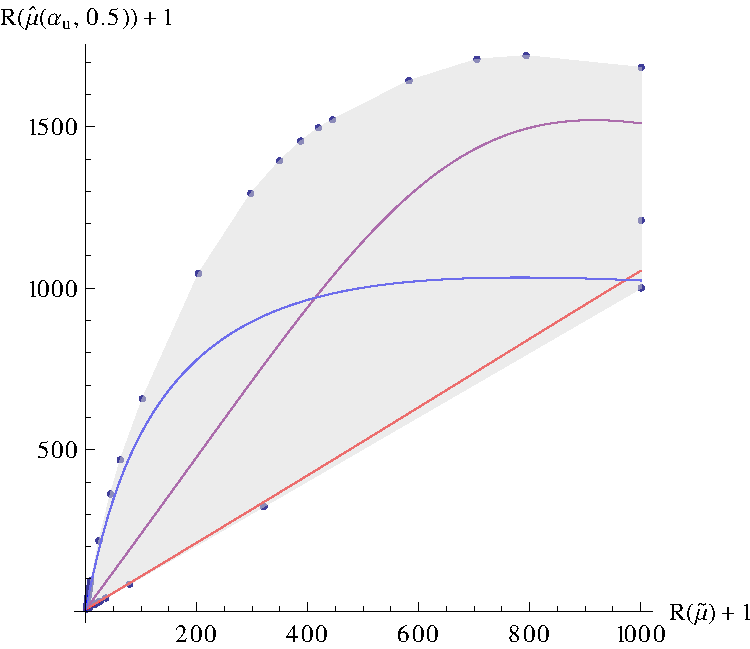
\includegraphics[width=3.0in]{figures/riFeasSet}
 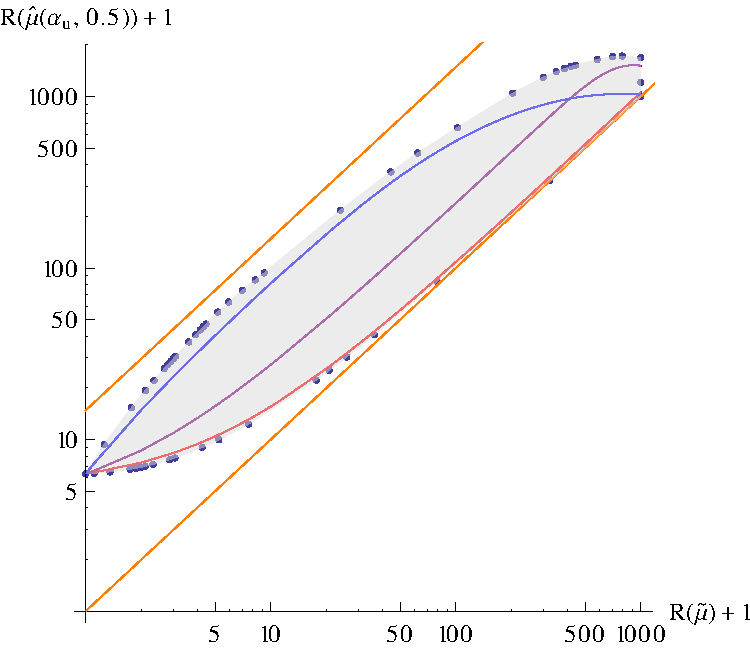
\includegraphics[width=3.0in]{figures/riFeasSetLog} }
 \vspace{0.2in}
 \end{figure}

 The two frames in Figure \ref{fig:riFeasibleSet} emphasize models with
 substantial signal (non-zero means) and those that are nearly black (most
 $\mu_j=0$).  The plot on the risk scale itself emphasizes the performance in
 models with substantial signal.  The vertical left edge of the feasible set
 shows the risk for saturated models in which $|\mu_j| > 1$; in this case, the
 risk of the oracle testimator is ${\cal R}_p(\tilde{\bmu}, \bmu) = p$.  The
 plot on the log scale emphasizes sparse models, the so-called nearly black
 context in which most $\mu_i = 0$.  In this frame, the line parallel to and
 above the diagonal is the risk-inflation boundary \eqn{eq:ri} that obtains for
 non-sequential estimators.  These bounds suggest that the worst case risk for
 the testimator should be about $1 + 2 \log p$ times the risk of the oracle.
  The feasible set calculations show that the risk of \uTest\ does indeed fall
 below this boundary, but that is not true of all estimators.  \ras{ Say more
 about the cool shape of the risk as the risk of the oracle goes to zero? }


 Curves within the feasible set show the risks of the two testimators that
 results if the means $\mu_{1:p}$ are determined by a two-point Bayesian model.
  Suppose that the stochastic process $\{\bmu\}$ that determines the means sets
 $\mu_j$ at random to some non-zero value $\mu^{*}$:
 \begin{equation}
    \mu_j = B_j \; \mu^{*}, \quad B_j  \iid \mbox{ Bernoulli}(\pi)  \;.
 \label{eq:muj}
 \end{equation}
 The smooth curves within the feasible set show the risks under this
 probabilistic model, with $\mu^{*}$ = 1.0 (red), 1.5 (magenta), or 3 (blue),
 and the probability of a non-zero mean varying over the range $10^{-6} \le \pi
 \le 1-10^{-6}$.  With $\mu^{*} = 1.0$, the risks nearly trace out the lower
 boundary of the feasible set. 


 Displays of several feasible sets within the same plot allow one to compare the
 effects of various choices.  As an example, Figure \ref{fig:univVsRI} considers
 the effect of lowering the initial wealth $w_0$ and payoff $\omega$ from 0.50
 down to smaller values, here 0.25 and 0.05.  The left frame on the scale of
 risks emphasizes the comparison in problems with greater levels of signal; the
 right frame on the log scale emphasizes sparse, nearly black models.  Within
 the context of testing, choosing $\al=0.05$ is the virtual default and an
 intuitive choice would be to similarly choose to control the false discovery
 rate at 0.05.  Unless one is very convinced that nature will play a nearly
 black strategy, however, this choice of $w_0 = \omega$ generates far greater
 risk than $w_0=0.25$ or 0.50.  With $w_0=0.05$, the risks even escape the
 bounds suggested by risk inflation in the non-sequential setting, shown here by
 points in the feasible set above the bound provided in \eqn{eq:ri}.  Because
 these plots show several feasible sets together, one can no longer interpret a
 point in the graph as representing a specific mean vector $\bmu$ that produces
 the shown risks.  Points within each feasible set indicate that there exists
 for that pair of estimators a mean vector that generates the shown risks, but
 at a given $(x,y)$ location, the mean vectors that produce the risks for the
 several feasible sets differ.

\begin{figure}
 \caption{ \label{fig:univVsRI} {\sl Feasible sets comparing the risk inflation
 oracle to the risk of the universal estimator \uTest with $w_0=0.05$, 0.25, and
 0.50 with $p$=1,000 tests on the scale of risks (left) or log risks (right).}
  }

 \vspace{0.1in}
 \centerline{
 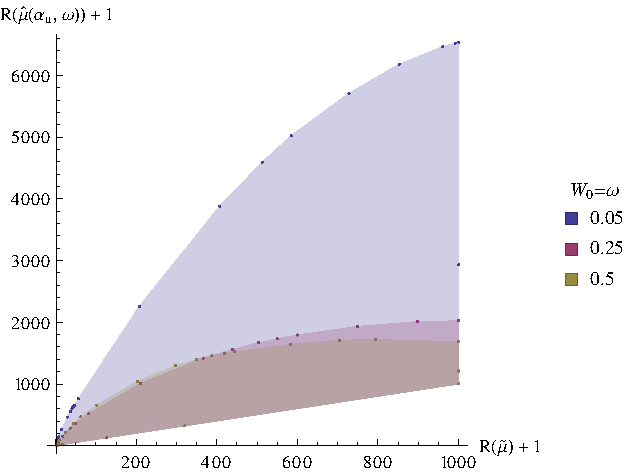
\includegraphics[width=3.5in]{figures/univVsRI}
 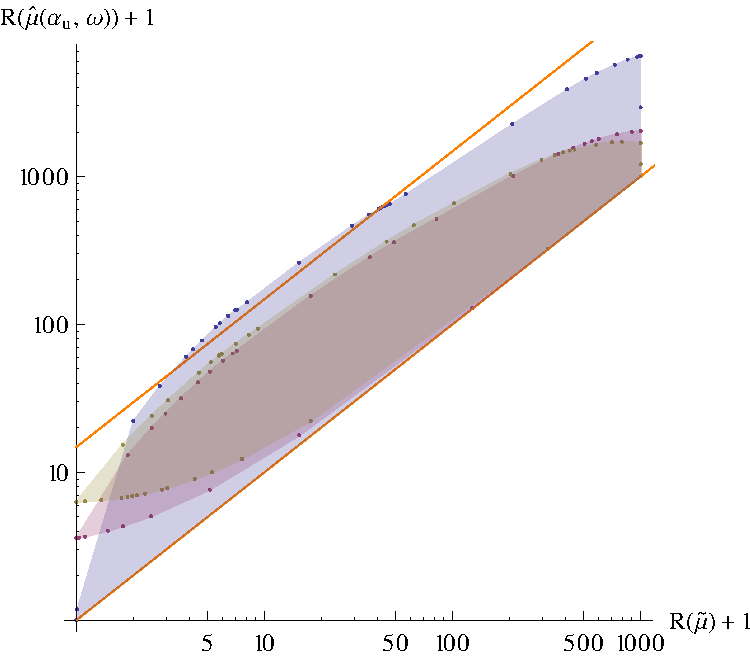
\includegraphics[width=3.0in]{figures/univVsRILog}    }
 \vspace{0.2in}
\end{figure}


 We have emphasized universal investing as defined by $\al_u(\cdot)$, and Figure
 \ref{fig:geom} offers a partial explanation for our choice.  Figure
 \ref{fig:geom} superimposes the feasible sets obtained by geometric investing
 $\al_g(\psi)$ defined in \eqn{eq:Ageo} versus the risk inflation testimator
 $\hat{\bmu}$.  The results are for a sequence of $p = 500$ tests.  In general,
 increasing the spending rate $\psi$ from 0.001 up to 0.01 improves the
 comparison, reducing the risk and shrinking the feasible set back toward the
 diagonal.  The feasible sets for $\psi=0.001$, 0.005, and 0.01 progressively
 move toward the diagonal, better competing with the risk-inflation testimator.
  The move to $\psi = 0.05$, however, goes too far.  The estimator essentially
 exhausts its alpha wealth before the testing is completed, and consequently its
 risk soars.  Because this geometric estimator must set $\hat\mu_j = 0$ when it
 has no remaining alpha wealth, its risk easily passes above the risk inflation
 boundary \eqn{eq:ri}.


\begin{figure}
 \caption{ \label{fig:geom} {\sl Comparison of the feasible sets for geometric
 investing rules defined by \eqn{eq:Ageo} with $p=500$ and rates $\psi=$ 0.001,
 0.005, 0.01, and 0.05.}  Spending down the wealth too quickly with $\psi=0.05$
 leads to excessive risk.  }

 \vspace{0.1in}
 \centerline{
   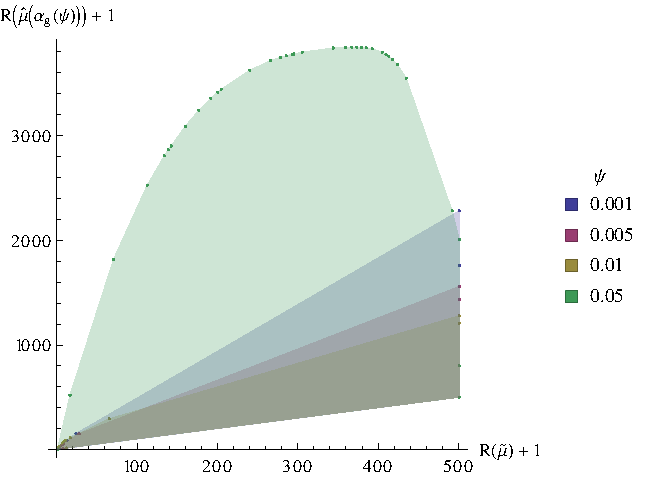
\includegraphics[width=3.5in]{figures/geom}     }
 \vspace{0.2in}
\end{figure}


%--------------------------------------------------------------------------
\section{ Computation }
%--------------------------------------------------------------------------


 We describe first the calculation of the feasible set ${\cal R}_p(\hat\mu(
 \al(\cdot), w_0, \omega), \tilde{\bmu})$ that contrasts an alpha investing
 estimator with the risk-inflation estimator $\tilde{\bmu}$.  The risk-inflation
 estimator has no wealth constraint; calculations need only track the wealth of
 the alpha investing estimator, which we abbreviate as $\hat{\bmu}$ with the
 understanding that it depends on the choice of the investing function
 $\al(\cdot)$, $w_0$, and $\omega$ throughout this section.  Let
 \begin{equation}
   {\cal U}^\theta(\hat{\bmu},\tilde{\bmu}) = 
       \max \evsub{\bmu} 
       \cos(\theta) R(\hat{\bmu}, \bmu) + \sin(\theta) R(\tilde{\bmu},\bmu) 
 \label{eq:U}
 \end{equation}
 denote the maximum expected value with respect to $\bmu$ of the weighted sum of
 risks defined by the angle $ 0 \le \theta \le 2 \pi$.  Let $\bmu^\theta$ denote
 the mean process that maximizes $U^\theta$.  The point
 $\evsub{\bmu^\theta}(R(\hat{\bmu}, \bmu), R(\tilde{\bmu}, \bmu))$ lies on
 the boundary of ${\cal R}_p(\hat{\bmu},\tilde{\bmu})$ where the feasible set is
 tangent to the line defined by the mixture weights in \eqn{eq:U}.  Plots that
 show the feasible set, such as Figure \ref{fig:riFeasibleSet}, highlight the
 boundary points that are explicitly computed.  By varying $\theta$ over the
 circle, we approximate the feasible set as the intersection of the resulting
 half-planes.

 
 We compute ${\cal U}^\theta$ via numerical backward induction.  This induction
 approximates the wealth of the alpha investing estimator along a grid.  The
 wealth grid $G$ spans the minimal attainable wealth ($w_0 - \sum_{j=1}^p
 \al_j$) to a maximum allowed wealth, which we set to $w_{\max} = 5$.  (Our
 results have not been sensitive to the choice of $w_max$ so long as it is
 substantially larger than $w_0 + \omega$.)  The wealth grid holds is
 `logarithmically' spaced at $N$ points, placing a finer grid with increments
 0.001 for small wealths below 0.02 and gradually wider grid as the wealth
 increases.  We insure that the grid includes an element $G_{k_0} = w_0$.


 The $p \times N$ matrix $U^{\theta}$ holds intermediate calculations of the
 expected value $\cal U$.  The rows in this matrix identify the hypothesis $H_j$
 and the columns index the position in the wealth grid $G$.  We fill $U^\theta$
 from the `bottom up' in a tail recursion.  At the completion of the
 calculations,
 \begin{eqnarray}
   U^\theta_{jk} &=&  \max_\mu \;\Bigl\{
     \cos(\theta) R(\hat\mu_{\al(G_k)}, \mu) + \sin(\theta) R(\tilde{\mu},\mu) \cr
     & &+ r_\mu\left(\al(G_k)\right) \;
          \left(c \,U^{\theta}_{j+1,k_c+1} + (1-c) U^{\theta}_{j+1,k_c}\right) \cr
     & & + (1- r_\mu\left(\al(G_k)\right) \; 
          \left(d \,U^{\theta}_{j+1,k_d+1} + (1-d) U^{\theta}_{j+1,k_d}\right)   
     \Bigr\}
 \label{eq:Ujk}
 \end{eqnarray}
 for the indices spanning $j=p, p-1,\ldots,1$ and $k = 1,\ldots,N$ and the
 boundary condition $U^\theta_{p+1,k} = 0$.  At the completion of the
 computation, ${\cal U}^\theta = U^{\theta}_{1,k_0}$.  The first line of
 \eqn{eq:Ujk} adds the contribution to the weighted risk from testing $H_j$ at
 the alpha level $\al(G_k)$.  The second line adds the expected subsequent risk
 if the test rejects $H_j$, which occurs with probability $r_\mu(\al(G_k))$.  If
 the test rejects, the alpha wealth increases to $G_k + \omega$.  This wealth is
 unlikely to match any $G_k$, so we linearly interpolate in the grid between
 positions $k_r$ and $k_r+1$ defined so that $G_{k_r} \le G_k + \omega \le
 G_{k_r+1}$ and $c = (\omega+G_k)/(G_{k_c+1}-G_{k_c})$.  Similarly, the third
 line of \eqn{eq:Ujk} adds the expected contribution if the testimator does not
 reject $H_j$ and its wealth falls to $G_k - \al(G_k)$.  

 \remark{ One need not store the full matrix $U^\theta$, but its use simplifies
 the description of the algorithm.  One only needs $U^\theta_{j+1,\cdot}$ when
 computing $U_{j,\cdot}$.  Such space saving becomes essential in problems that
 must track a larger state space.  Note also that one can cache the indices and
 weights ($k_c, c$ and $k_d, d$) prior to the recursion because these can be
 determined from the grid positions and $\omega$ and remain fixed throughout the
 backward recursion.}


 The feasible set that compares the testimators defined by two alpha investing
 rules $\al(\cdot)$ and $\beta(\cdot)$ requires a more complex recursion that
 must track the wealths of both.  The linear grid $G$ remains, but the matrix
 $U^\theta$ defined in \eqn{eq:Ujk} becomes a three dimensional tensor of size
 $p \times N \times N$.  The calculation is essentially a more messy version of
 \eqn{eq:Ujk} but for one nuance that we want to emphasize.  To simplify the
 presentation, we suppress the linear interpolation and pretend that all of the
 concerned wealths are represented in the wealth grid.  If the alpha investing
 rule $\al(\cdot)$ with wealth $G_k$ rejects $H_j$, its wealth goes from $G_k$
 to $G_{k+}$; if it fails to reject, its wealth falls to $G_{k-}$.
  Similarly, we use $\ell+$ and $\ell-$ for the positions for the rule defined
 by $\beta(\cdot)$.  The recursion then can be written as recursion as
 \begin{eqnarray}
   U^\theta_{jk\ell} &=&  \max_\mu \;\Bigl\{
     \cos(\theta) R(\hat\mu_{\al(G_k)}, \mu) 
       + \sin(\theta) R(\hat\mu_{\beta(G_\ell)},\mu) \cr
     & & + r_\mu\left(\al(G_k)\right) \; U_{j+1,k+,\ell+} 
         + \left[ r_\mu(\beta(G_\ell)) - r_\mu(\al(G_k)) \right] \, U_{j+1,k-,\ell+} \cr
     & & + \left[1-r_\mu(\beta(G_\ell))\right] \, U_{j+1,k-,\ell-} \, \Bigr\}\;,
 \label{eq:Ujkl}
 \end{eqnarray}
 where we assume for convenience that $\al(G_k) < \beta(G_\ell)$ and the
 boundary condition $U_{p+1,\cdot,\cdot}^\theta= 0$.  The first line in
 \eqn{eq:Ujkl} is the expected risk produced by the test of $H_j$, and following
 summands denote the subsequent maximum expected contributions to the risk if
 both reject, if only the rule with the larger alpha level rejects, and if
 neither rejects.  The point of writing this out is to emphasize these
 testimators see the same data, not independent samples.  Hence, $\al(G_k) <
 \beta(G_\ell)$ implies that if the first rule $\al(\cdot)$ rejects $H_j$, then
 the second rule must also reject $H_j$ because it tests the same hypothesis
 with a larger alpha level.  


%--------------------------------------------------------------------------
\section{ Discussion }
%--------------------------------------------------------------------------


 Return to model selection.

  Suppose one has a collection of $p$ variables $X_1, \ldots, X_p$ to consider as
 explanatory variables in the classical linear regression model
 \begin{equation}
   Y_i = \beta_0 + \beta_1 X_{i1} + \cdots + \beta_p X_{ip} + \ep_i, 
     \qquad \ev \ep_i = 0, \Var(\ep_i)=\sigma^2,  \quad i = 1,\ldots,n\;.
 \label{eq:regr}
 \end{equation}
 As a method for picking a model, subset selection (sometimes called $L_0$
 selection) in effect tests the hypotheses $H_j: \beta_j = 0, \; j = 0, 1, \ldots, p$.
  Let $\gamma_j = \pm 1$ denote those $\beta_j \ne 0$, and let $\hat\gamma_j =
 \pm 1$ identify the rejected hypotheses.  The explanatory variable $X_j$
 appears in the fitted model if $\hat\gamma_j = 1$ and is excluded otherwise
 (hence estimating $\beta_j$ = 0).  We insert an intercept in all models (as
 needed by risk inflation below) and so set $\gamma_0=\hat\gamma_0 = 1$.  The
 vectors $\gamma = (1, \gamma_1, \ldots, \gamma_p)'$ and $\hat\gamma = (1,
 \hat\gamma_1, \ldots, \hat\gamma_p)'$ collect these indicators.


Alpha investing can mimic regular testing procedure by revisiting the test of
prior hypotheses. 

Improve the estimator by shrinkage.



 One might also use accumulated alpha wealth as a measure of the performance, and
 this provides a more useful metric of performance, particularly when competing
 against the oracle.  If maximizing alpha wealth, then the oracle loses the
 amount bid and chooses $\mu_j$ to maximize $r_{\mu_j}(\al)-\al$ rather than
 $r_{\mu_j}(\al)$ alone.  This perspective would not only capture aspects of
 rejecting hypotheses, it also anticipates having resources to test future
 hypotheses.  Such consideration is appropriate, however, only in the context of
 testing a larger collection of hypotheses than considered here.

 \ras{ Things left to do:}
 \begin{enumerate}

 \item Graphs of envelope that suggest that alpha wealth is a decent proxy for
 risk, at least better than something like FDR, number rejects - constant times
 number false rejects.

 \item What does the steady state look like.  If take the envelope for 250 and
 double to get for 500, is that close to correct for the risk?

 \item Comment on the value of saving if hope to compete with a universal
 bidder.

 \item  Talk about simulating the mean processes; or save for another day? 
 
\item {\bf Stationarity} of the associated wealth process, perhaps using results
 from \citet{chanTong94} for the geometric ergodicity of the process in the
 universal case.

\end{enumerate}



%--------------------------------------------------------------------------
\section{ Bibliography }
\section*{Acknowledgement}
%--------------------------------------------------------------------------

The authors thank ...


%--------------------------------------------------------------------------
% References
%--------------------------------------------------------------------------

\bibliography{../../../../references/stat}
\bibliographystyle{../../bst/asa}

\end{document} %==========================================================
